\section{Theoretical background}

\subsection{Group theory}
    \textbf{Group} $G$ is a set together with binary operation $\left(G, \bullet \right)$ satisfying
    following axioms:
    \begin{enumerate}
        \item Closure: for any $g, h \in G$, $g \bullet h \in G$
        \item Associativity:  $g\bullet \left(h \bullet j \right) =
                    \left(g \bullet h \right) \bullet j$ for any $g,h,j \in G$
        \item Identity: there exists a neutral element $e$ such that
                $e \bullet g = g \bullet e = g$ for any $g \in G$
        \item Inverse element: for every $g \in G$ exists element $h \in G$ such that
                $g \bullet h = h\bullet g = e$. The element inverse to $g$ is usually
                written as $g^{-1}$
    \end{enumerate}
    \par Group $G$ might also posses additional structure. A \textbf{topological group}
        is a group together with a topology on G, such that $G$'s binary operation:\\
        \hspace*{0.5cm} $\bullet: G \times G \to G, \left(g,h \right) \mapsto g\bullet h$ \\
        and inversion map: \\
        \hspace*{0.5cm} ${}^{-1}: G \to G, g \mapsto g^{-1}$ \\
        are continuous. Additionally if the underlying topological structure
        is some smooth n-manifold and both maps are smooth, the group is called
        \textbf{Lie group}. Familiar examples of Lie groups include translation group
        $\left( \mathbb{R}^n, + \right)$ - set of real vectors with addition or
        $\left(GL(n,\mathbb{R}), \cdot \right)$ - set of real $n \times n$ matrices of nonzero determinant
        with multiplication.\\\par
        Just as we can form functions between sets assigning elements of one set to
        the elements of other, it's possible to construct functions between groups.
        Typically we are interested in functions preserving to some extent the group structure,
        that is of the form.
        \begin{equation}
            f:G \to H, \hspace{1cm} f(x\bullet y) = f(x) \ast f(y)
        \end{equation}
        where $\bullet$ is the binary operation in group $G$ and $\ast$ is the binary operation
        in group $H$. Such functions are called \textbf{group homomorphisms}.
        Bijective homomorphism is called \textbf{isomorphism}.\\

        In this work we are mainly interested in groups in context of their actions
        on 3D tensors. Given a group $G$ and set $X$ we define a
        \textbf{group action} of $G$ on $X$ as a function
        \begin{equation}
            \theta: G \times X \to X
        \end{equation}
        (with $\theta(g,x)$ often written as $g\cdot x$) satisfying following axioms:
        \begin{enumerate}
            \item Identity: $e \cdot x = x$ for every $x \in X$, where $e$ is the neutral element
                    of $G$
            \item Compatibility: $g \cdot \left(h \cdot x\right) =
                \left(g \bullet h \right) \cdot x$ for all $g$ and $h$ in $G$ and $x$ in $X$
        \end{enumerate}
        The simplest possible group action is the trivial group action, that is
        $g\cdot x = x$ for any $g$ and $x$. Familiar nontrivial examples include isometries
        of $\mathbb{R}^n$, e.g.
        translations - action of $\left(\mathbb{R}^n,+\right)$ given by $v \cdot x = v+x$ or
        rotations - action of $SO(n,\mathbb{R})$ given by $r \cdot x = Rx$ where
        $R$ is matrix representation of rotation and
        multiplication on the right is matrix-vector multiplication.\\
        Now suppose we are given some function $f:G\to \mathbb{R}^n$.
        We can define natural action of $G$ on set of such functions by:
        \begin{equation}
            (g\cdot f)(x) = f(g^{-1}\bullet x)
        \end{equation}
        It's a group action because:
        \begin{align*}
            & (e\cdot f)(x) = f(e\bullet x) = f(x) \\
            & \mbox{and} \\
            & ((g\bullet h) \cdot f)(x) = f((g\bullet h)^{-1} \bullet x) =
            f(h^{-1}\bullet g^{-1} \bullet x) = (h\cdot f)(g^{-1} \bullet x) =
            (g\cdot(h \cdot f))(x)
        \end{align*}








\subsection{Equivariant and invariant neural networks}
    \subsubsection{Equivariant and invariant maps}
    \label{sec:theoretical_equiinv}
    \hspace{0.5cm}
     Key properties of neural networks in regard to group actions are equivariance and invariance.
        These can be abstractly defined as follows: \par
        Let group $G$ act on sets $X$ and $Y$. We call function $f: X \rightarrow Y$ equivariant
        with respect to action of $G$ if for all $g \in G$ and $x \in X$
        \begin{equation}
            f(g \cdot x) = g \cdot f(x)
        \end{equation}
        In turn, we call $f$ invariant with respect to action of $G$
        \begin{equation}
            f(g \cdot x) = f(x)
        \end{equation}
        In fact invariance is a special case of equivariance where action of $G$ on $Y$ is trivial.
        It's however conceptually cleaner to make distinction between both properties.
        Intuitively equivariance tells us that when input changes, the output changes accordingly
        and invariance -- that action of G has no effect on output.\par
            If we want to construct a neural network $\mathcal{N}$ equivariant to some
        specified group action, we need to make sure each of it's layers is equivariant.
        If we treat $\mathcal{N}$ as a series of functions $f_0,f_1,...,f_n$, then
        \begin{align*}
            \mathcal{N}(g \cdot x) &=
            f_n \circ f_{n-1} \circ \cdots \circ f_1 \circ f_0(g\cdot x)  \\
            &= f_n \circ f_{n-1} \circ \cdots \circ f_1 \circ \left( g \cdot f_0(x) \right) \\
            &= \cdots \\
            &= g \cdot f_n \circ f_{n-1} \circ \cdots \circ f_1 \circ f_0(x) \\
            &= g \cdot \mathcal{N}(x)
        \end{align*}
        where $g\cdot x$ is the action of $g$ on $x$. Often we don't want the network
        to be fully equivariant; the desired extent of equivariance depends on the task.
        For problems of image-to-image type like segmentation full equivariance is desirable.
        However for problems where the input data gets more and more ``squished'' in consecutive layers,
        we need to break equivariance at some point. Like for example in classification,
        where final layers are often fully connected and not equivariant. \par
        The easiest way to assert the network is invariant to some transformation
        is making it's very first layer $f_0$ invariant, then:
        \begin{align*}
            \mathcal{N}(g\cdot x)
            &= f_n \circ f_{n-1} \circ \cdots \circ f_1 \circ f_0(g\cdot x)  \\
            &= f_n \circ f_{n-1} \circ \cdots \circ f_1 \circ f_0(x) \\
            &= \mathcal{N}(x)
        \end{align*}
        Equivalently one can make the couple first layers equivariant and a single layer
        following them invariant. For example if $f_0$ is equivariant and $f_1$ invariant we get:
        \begin{align*}
            \mathcal{N}(g\cdot x)
            &= f_n \circ f_{n-1} \circ \cdots \circ f_1 \circ f_0(g\cdot x)  \\
            &= f_n \circ f_{n-1} \circ \cdots \circ f_1 \circ \left( g \cdot f_0(x) \right) \\
            &= f_n \circ f_{n-1} \circ \cdots \circ f_1 \circ f_0(x) \\
            &= \mathcal{N}(x)
        \end{align*}
        and the network is again invariant.

    \subsubsection{GCNN}
    The primary example of equivariant neural networks are convolutional neural
    networks which are (roughly) equivariant to translations. The $4$ basic
    components of CNN are convolutional layers, pooling layers, normalization
    layers and activation functions.  These common building are approximately
    equivariant to translations:
    \begin{itemize}
        \item Convolutional layer is
            equivariant outisde of image's borders. The border effects can to
            some extent be fixed by padding image with values present in the
            border or their avarages.
        \item Max pooling layer is locally invariant -- that is small translations don't
            affect the layer's output, but translations which are multiplicities
            of window's size cause equivariant behaviour.
            In average pooling local behaviour is more
            complicated, but they are also equivariant to window-sized
            translations.
        \item Usual normalization schemes like batch or instance
            normalization depend on global statistics
            like mean and standard deviation which change slightly during
            translation so their are not exactly equivariant. However given
            proper padding method these changes can be very small if
            translation is not too big.
        \item Activation functions are applied pointwise so, they are
            perfectly equivariant outside borders.
    \end{itemize}
    Of course the most crucial parts of CNN are convolution layers. At each
    layer CNN takes as input 3-dimensional tensor which can be thought of as a
    stack of functions $f:\mathbb{Z}^2\to\mathbb{R}^C$ where $C$ is number of channels.
    Convolutional layer correlates it with a set of filters $\psi^i$
    and each filter can also be thought of as a stack of functions
    $\psi^i:\mathbb{Z}^2\to\mathbb{R}^C$:
    \begin{equation}
        \label{eq:cnn}
        (f\star\psi^i)(x) = \sum_{y\in\mathbb{Z}^2}\sum_{c=1}^C
        f_c(y)\psi_{c}^{i}(y-x)
    \end{equation}

    By generalizing convolutions and architecture of CNNs we would like to
    construct models
    equivariant or invariant to some specified set of image transformations.
    One of the earliest works on this problem appeared in \cite{cohen2016}. There
    the so called \textit{Group Equivariant Convolutional Neural Networks}
    (G-CNNs) equivariant to possibly any discrete set of transformations were
    proposed. Their main idea is generalizing the convolution layer by
    lifting tensors the network operates on to higher dimensions.
    Just like traditionally the last two
    dimensions encode height and width, these new dimensions can
    encode information about the chosen group of transformations. These higher
    dimensional tensors are then thought of as stacks of functions
    $f:G\to\mathbb{R}^C$. Pictures \ref{fig:p4_rot} and \ref{fig:p4m_rot} show
    feature maps for group of translations and rotations and for group of
    translations, rotations and reflections respectively. Convolutional filters have similar
    shape, just their heights and widths are smaller.
    \begin{figure}[h]
        \centering
        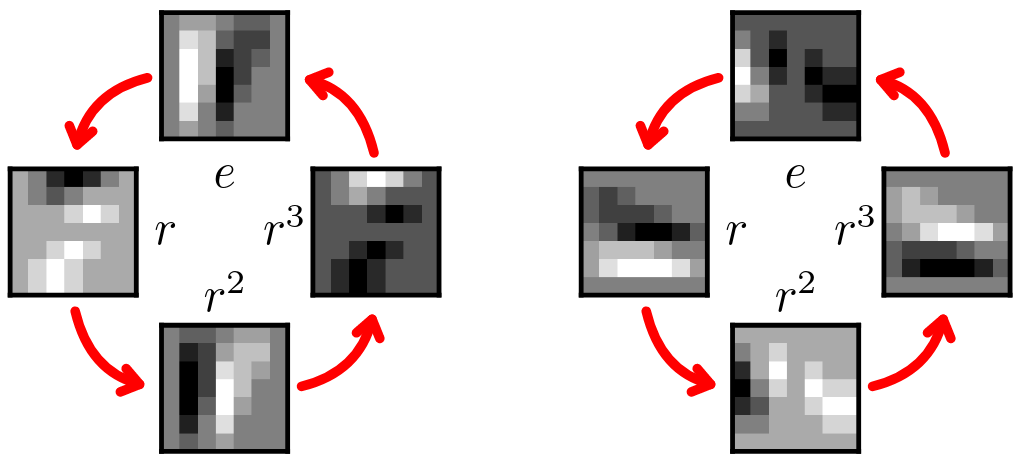
\includegraphics[width=0.7\textwidth]{p4_rot}
        \label{fig:p4_rot}
    \end{figure}
    \begin{figure}[h]
        \centering
        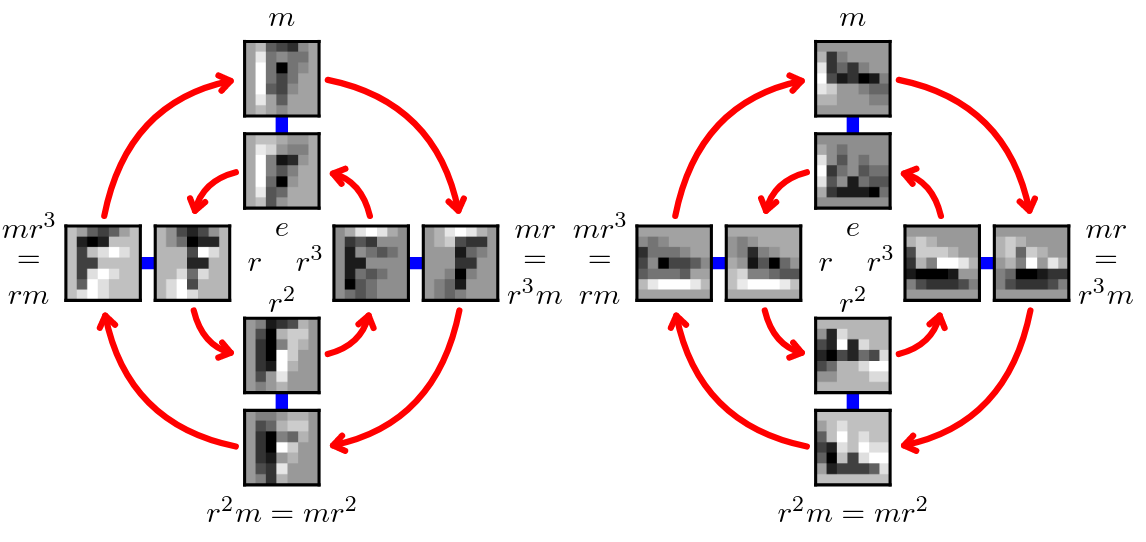
\includegraphics[width=0.7\textwidth]{p4m_rot}
        \label{fig:p4m_rot}
    \end{figure}

    \textbf{Lift} operation transforms tensor from function stack on $\mathbb{Z}^2$
    to function stack on group $G$:
    \begin{equation}
        \label{eq:gcnn-lift}
        (f\star\psi^i)(g) = \sum_{y\in \mathbb{Z}^2}\sum_{c=1}^C
        f_c(y)\psi_{c}^{i}(g^{-1}y)
    \end{equation}
    Once the input tensor is lifted, in consecutive convolutional layers it
    undergoes \textbf{group convolutions}:
    \begin{equation}
        \label{eq:gcnn}
        (f\star\psi^i)(g) = \sum_{y\in G}\sum_{c=1}^C
        f_c(y)\psi_{c}^{i}(g^{-1}y)
    \end{equation}
    Note that while in equation \ref{eq:cnn} computation is done by sliding
    $y$ on $\mathbb{Z}^2$, in equation \ref{eq:gcnn} it's replaced by more
    general iteration on all group elements. If we replace $G$ by $\mathbb{Z}^2$
    and set $g=x$ we obtain equation \ref{eq:cnn} back since in $\mathbb{Z}^2$,
    $x^{-1}$ is just $-x$. We can prove operator defined by equation
    \ref{eq:gcnn} is equivariant to action of any element $h$ of $G$:
    \begin{align*}
        ((h\cdot f)\star\psi)(g) & =
        \sum_{y\in G}\sum_{c=1}^C f_c(h^{-1}y)\psi_{c}(g^{-1}y)\\
        & = \sum_{hy\in G}\sum_{c=1}^C f_c(y)\psi_{c}(g^{-1}hy)\\
        & = \sum_{hy\in G}\sum_{c=1}^C f_c(y)\psi_{c}((h^{-1}g)^{-1}y)\\
        & = (f\star\psi)(h^{-1}g) &  \\
        & = (h\cdot(f\star\psi))(g)
    \end{align*}
    The proof goes similarly for equation \ref{eq:gcnn-lift}.

    The ideas contained in \cite{cohen2016} were further generalized to new
    domains, new possible group of transformations and neural network
    architectures. \cite{bekkers2019, lieconv} propose general frameworks for
    GCNNs equivariant to any Lie group whereas \cite{cohen2016} only really
    touched on finite groups. That's important since many natural
    transformations of data are continuous and often have structure of Lie group
    like group of all rotations of plane ($SO(2)$), rotations of sphere
    ($SO(3)$) or scaling of images $(R_+, \times)$.

    %TODO: write about each generalization, cite and insert some pictures

\subsection{Image symmetries}
    \label{sec:transformations}
    In this section we define and generalize symmetries of images that we wish
    neural networks to respect. First we describe
    properties related to lightning in image - contrast,
    brightness, color balance and gamma correction. Then geometric operators -
    rotations, scaling and shear - are presented.
    Throghout this section and for the rest of the work,
    ``image'' is understood to be an array of
    floating point numbers in range $\left[0;1\right]$ of shape $\left(3, H,
    W\right)$.
    \subsection{Lightning operators}
    \subsubsection{Contrast}
    \newcommand\mcc{\mathcal{C}}
        The usual formula for changing image's contrast by factor of $a$ is
        \begin{equation}
            \label{eq:contrast_old}
        C_a(X) = \mathit{CLIP}\left(a\cdot X + (1-a) \cdot E\left[ \frac{w_1X_r
        + w_2X_g + w_3X_b}{w_1+w_2+w_3}\right]   \right)
        \end{equation}
        where
        $\mathit{CLIP}$ is function clipping values to $\left[0;1\right]$ range,
        $X_r, X_g$ and $X_b$ are red, green and blue channels of the image and
        the expectation on the right is mean value of grayscale version of
        image.  Grayscale is understood to be a weighted average of image's
        channels.  Changing the contrast by factor of $1$ has no effect, using
        the factor of $2$ is supposed to double the contrast, factor of $0.5$
        halves the contrast, etc.  This definition however is not suitable for
        usage in the context of neural networks.  First of all it assumes the
        tensor has 3 channels, while we would like to have a definition
        independent of number of channels. The concept of green channel or red
        channel also doesn't exist for tensors with more channels. Therefore we
        choose to generalize the definition by replacing weighted average with
        usual average. The second problem is clipping values. Working only with
        values in range $\left[0;1\right]$ at all times would make training a
        neural network a lot harder and perhaps significantly diminish it's
        performance. To avoid these effects we entirely give up on clipping
        values.  The final formula for changing contrast is following:
        \begin{equation}
            \label{eq:contrast}
            \mathcal{C}_a(x) = ax + (1-a) \mu_x
        \end{equation}
        where $\mu_x$ is the average value of whole tensor. It's however worth
        noting, that removing the clipping changes the general behavior of the
        transformation.  While it remains more or less unchanged for values of
        $a$ close to $1$, differences grow as me move further away from identity
        transformation.
        % TODO: plot of difference between original definition and the adopted definition

        This operator possesses a number of interesting properties:
        \begin{itemize}
            \item $\mathcal{C}_a$ is linear operator on vector space of images of fixed size:
                \begin{align*}
                    & \mathcal{C}_a(x+y) =
                    a(x+y) + (1-a)\mu_{x+y} =
                    ax + ay +(1-a)\mu_x +(1-a)\mu_y =
                \mathcal{C}_a(x) + \mathcal{C}_a(y) \\
                    & \mathcal{C}_a(\lambda x) = a\lambda x + (1-a)\mu_{\lambda x} =
                    \lambda ax + (1-a)\lambda\mu_x = \lambda(ax + (1-a)\mu_x) =
                    \lambda \mathcal{C}_a(x)
                \end{align*}

            \item Under map composition, set
                $\mathcal{C} = \left\{\mathcal{C}_a | a\in \mathbb{R}_+\right\}$
                forms a Lie group isomorphic to $\left(R_+,\cdot \right)$ -- set of
                positive real numbers with multiplication:
                \begin{enumerate}
                    \item Closure:\\
                        $\mathcal{C}_a\circ \mathcal{C}_b(x) =
                \mathcal{C}_a(bx + (1-b)\mu_x) =
                abx + a(1-b)\mu_x + (1-a)\mu_{bx+(1-b)\mu_x} =
                abx + a(1-b)\mu_x + (1-a)b\mu_x + (1-a)(1-b)\mu_x=
                abx + (1-ab)\mu_x =
                \mathcal{C}_{ab}(x)$
                    \item Associativity:\\
                        $ \mcc_a \circ(\mcc_b \circ \mcc_c(x)) =
                            \mcc_a(\mcc_{bc}(x)) = \mcc_{abc}(x) =
                                \mcc_{ab}\circ\mcc_c(x) = (\mcc_a \circ \mcc_b) \circ\mcc_c(x)$
                    \item Identity:\\
                        $\mcc_1\circ\mcc_a(x) = \mcc_a\circ\mcc_1(x) =
                            \mcc_a(x)$
                    \item Inverse element:\\
                        $\mcc_a\circ\mcc_{a^{-1}}(x) = \mcc_{a^{-1}}\circ\mcc_a(x) = \mcc_1(x)$
                \end{enumerate}
                The homomorphism is simply $h: \mcc_a \mapsto a$
                $$ h(\mcc_a)h(\mcc_b) = ab = h(\mcc_{ab})$$
                It is bijective so it's isomorphism.

            \item Equation \ref{eq:contrast} defines a group action of $\mcc$ on space of images:
                $\mcc_1 \cdot x = 1x + (1-1)\mu_x = x$ and checking the compatibility axiom
                is the same as checking the closure axiom above.
            \item $\mcc_n$ increases standard deviation of image $n$ times:\\
                $\sigma(\mcc_n(x)) = \sigma(nx + (1-n)\mu_x) = \sigma(nx) = n\sigma(x)$
        \end{itemize}
        \par Visually the difference between operators using weighted and unweighted
        averages is small. Picture \ref{fig:contrast_pics} shows series of
        photographies from STL10 dataset with with varying contrast changes.

        \newcommand{\contrastpic}[3]{
            \begin{subfigure}{#3\textwidth}
                \includegraphics[width=\linewidth]{contrast_#1/#2}
            \end{subfigure}}
        \newcommand{\contrastpiccaption}[4]{
            \begin{subfigure}{#3\textwidth}
                \includegraphics[width=\linewidth]{{contrast_#1/#2}.jpg}
                \caption*{$a=#4$}
            \end{subfigure}}

        \begin{figure}[h]
            \centering
            \foreach \n in {0_1, 0_25, 0_5, 1, 2, 4,10}
                {\contrastpic{default}{0temp\n}{0.12}} \\
            \foreach \n in {0_1, 0_25, 0_5, 1, 2, 4,10}
                {\contrastpic{custom}{0temp\n}{0.12}} \\[1em]
            \foreach \n in {0_1, 0_25, 0_5, 1, 2, 4,10}
                {\contrastpic{default}{121temp\n}{0.12}} \\
            \foreach \n in {0_1, 0_25, 0_5, 1, 2, 4,10}
                {\contrastpic{custom}{121temp\n}{0.12}} \\[1em]
            \foreach \n in {0_1, 0_25, 0_5, 1, 2, 4,10}
                {\contrastpic{default}{105temp\n}{0.12}} \\
            \foreach \n in {0.1, 0.25, 0.5, 1, 2, 4,10}
                {\contrastpiccaption{custom}{105temp\n}{0.12}{\n}}

        \caption{Differences between weighted and unweighted contrst change
            operator. Top rows: $C_a$ operator (equation \ref{eq:contrast_old}.
            Bottom rows: $\mcc_a$ operator (equation \ref{eq:contrast} with
            clipping).}
        \label{fig:contrast_pics}
        \end{figure}


    \subsubsection{Brightness}
        Change in image brightness is defined similarly to change in contrast, except
        the subtraction of image's mean is skipped:
        \begin{equation}
            \label{eq:bright_old}
            B_a(X) = \mathit{CLIP}\left(aX\right)
        \end{equation}
        Again omitting the clipping, the brightness change operator is defined simply as
        \begin{equation}
            \label{eq:bright}
            \mathcal{B}_a(x) = ax
        \end{equation}
        All properties characterising the $\mcc$ operators listed above
        are also true for the set $\mathcal{B} = \{\mathcal{B}_a | a>0 \}$.
        It's worth noting, that in this case removing the clipping step doesn't change
        the definition so significantly. In fact both formulas agree as long as $a\leq 1$,
        that is as along as brightness is not increased.
        Picture \label{fig:brightness_pics} shows images with brightness varying
        according to equation \ref{eq:bright_old}.


        \newcommand{\brightnesspic}[2]{
            \begin{subfigure}{#2\textwidth}
                \includegraphics[width=\linewidth]{{brightness/#1}.jpg}
            \end{subfigure}}
        \newcommand{\brightnesspiccaption}[3]{
            \begin{subfigure}{#2\textwidth}
                \includegraphics[width=\linewidth]{{brightness/#1}.jpg}
                \caption*{$a=#3$}
            \end{subfigure}}

        \begin{figure}[h]
            \centering
            \foreach \n in {0.1, 0.25, 0.5, 1, 2, 4,10}
                {\brightnesspic{0temp\n}{0.12}} \\
            \foreach \n in {0.1, 0.25, 0.5, 1, 2, 4,10}
                {\brightnesspic{121temp\n}{0.12}} \\
            \foreach \n in {0.1, 0.25, 0.5, 1, 2, 4,10}
                {\brightnesspiccaption{105temp\n}{0.12}{\n}}

        \caption{Images from STL10 dataset with brightness changed with operator
            $B_a$.}
        \label{fig:brightness_pics}
        \end{figure}


        %TODO: insert the plot of mean value of transformed image depending on change
        % brightness




    \subsubsection{Color balance}
        Suppose we are given a 3-channel image represented as a list of channels
        $\left[ X_r, X_g, X_b\right]$. Then the operator changing the color balance
        to the balance corresponding to the temperature $T$ is defined as
        \begin{equation}
            \mathcal{W}_T \left(\left[ X_r, X_g, X_b \right]\right) =
            \left[T_r X_r, T_g X_g, T_b X_b \right]
        \end{equation}
        where $T_r, T_g, T_b$ are RGB components corresponding to temperature $T$.
        For example for $T=1000K$, $T_r, T_g$ and $T_b$ equal $1, 0.0401$ and $0$ respectively.
        $T$ ranges from $1000K$ to $40000K$ with steps of $100$
        though there is not much change after the $15000$ threshold.
        Figure \ref{fig:color_balance} shows part of possible temperature spectrum
        together with colors characterising temperatures in terms of uint8 RGB triplets.
        Picture \ref{fig:cb_pics} shows images with varying color balance.

        \begin{figure}[h]
            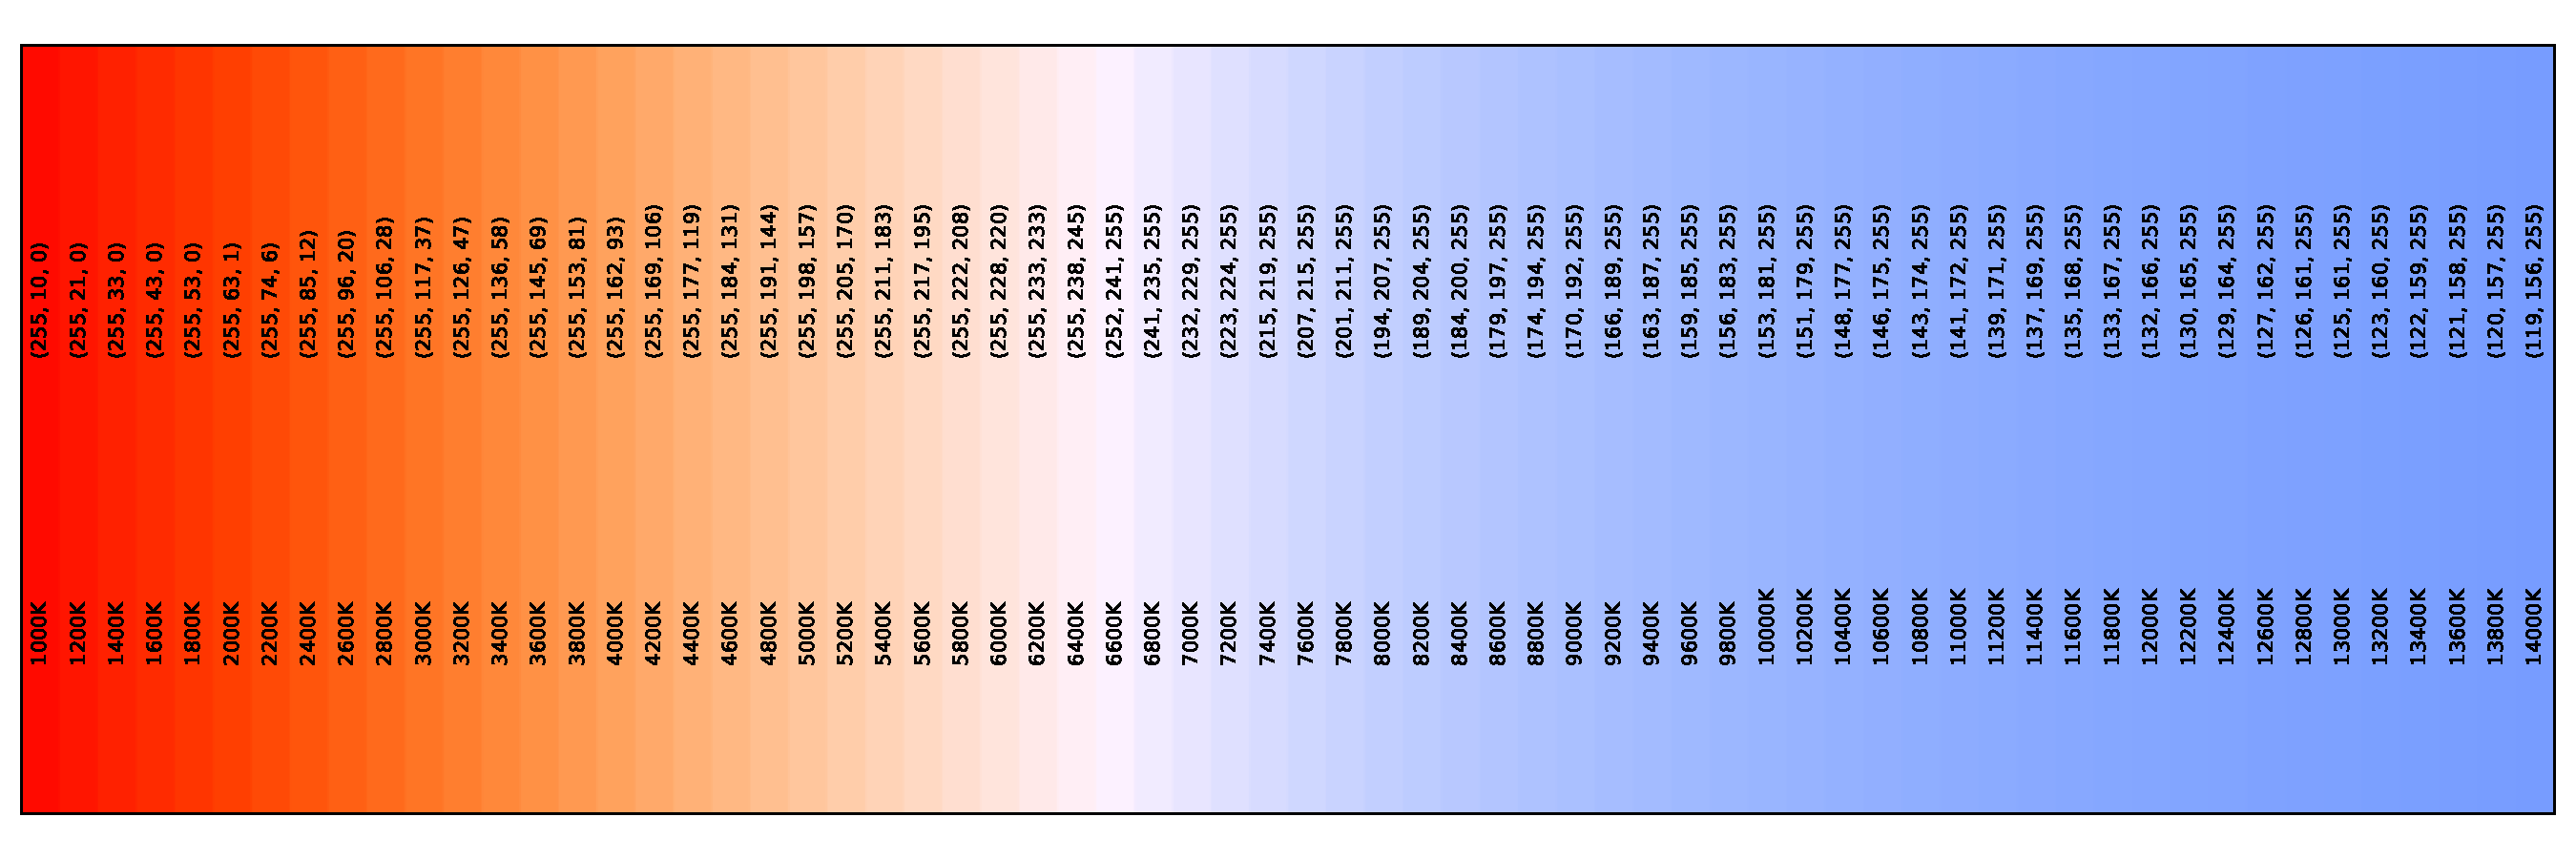
\includegraphics[width=\textwidth]{color_balance}
            \caption{}
            \label{fig:color_balance}
        \end{figure}

        \newcommand{\cbpic}[2]{
            \begin{subfigure}{#2\textwidth}
                \includegraphics[width=\linewidth]{{color_balance/#1}.jpg}
            \end{subfigure}}
        \newcommand{\cbpiccaption}[3]{
            \begin{subfigure}{#2\textwidth}
                \includegraphics[width=\linewidth]{{color_balance/#1}.jpg}
                \caption*{$T=#3K$}
            \end{subfigure}}

        \begin{figure}[h]
            \centering
            \foreach \n in {1000, 3000, 5000, 7000, 9000}
                {\cbpic{0temp\n}{0.18}} \\
            \foreach \n in {1000, 3000, 5000, 7000, 9000}
                {\cbpic{121temp\n}{0.18}} \\
            \foreach \n in {1000, 3000, 5000, 7000, 9000}
                {\cbpiccaption{105temp\n}{0.18}{\n}}

        \caption{Images from STL10 dataset with color balance changed with operator
            $\mathcal{W}_T$.}
        \label{fig:cb_pics}
        \end{figure}

        Unlike contrast or brightness, the color balance is inherently
        bound to colors of image, so it's very hard to come up with reasonable
        generalization to higher dimensions which would allow us to measure
        equivariance. We choose not to do that and instead only construct
        networks invariant to changes in color balance.

    \subsubsection{Gamma correction}

    \subsubsection{Rotation}
        When speaking of image rotating, we typically mean rotation around
        image's center. In coordinate system with $(0,0)$ representing the
        center, rotation of coordinates
        can be represented as an element of $SO(2)$ group - $2\times2$ matrix of
        the form
        $$\mathcal{R}_\theta = \begin{bmatrix}
                \cos\theta & -\sin\theta \\
                \sin\theta &  \cos\theta
            \end{bmatrix}$$
        which transforms coordinates (2d vectors) by matrix multiplication.
        After rotating coordinates pixels of original image need to be resampled
        in some way, which slightly distors the picture unless the rotation angle
        is a multplie of $90\degree$. If we want rotations to preserve all
        information present in picture
        we need to take care of appriopriate
        expansion of borders and possible padding with 0s.
        It's also important from more theoretical point of view - expansion
        assures rotations compose nicely, that is form a group
        action on the space of images.
        Figure
        \ref{fig:rotation_pics} illustrates neccesity of border expansion.
        Lack of expansion causes rotation composition to lose part of
        information which moves outisde the border.

        \begin{figure}[h]
            \centering
            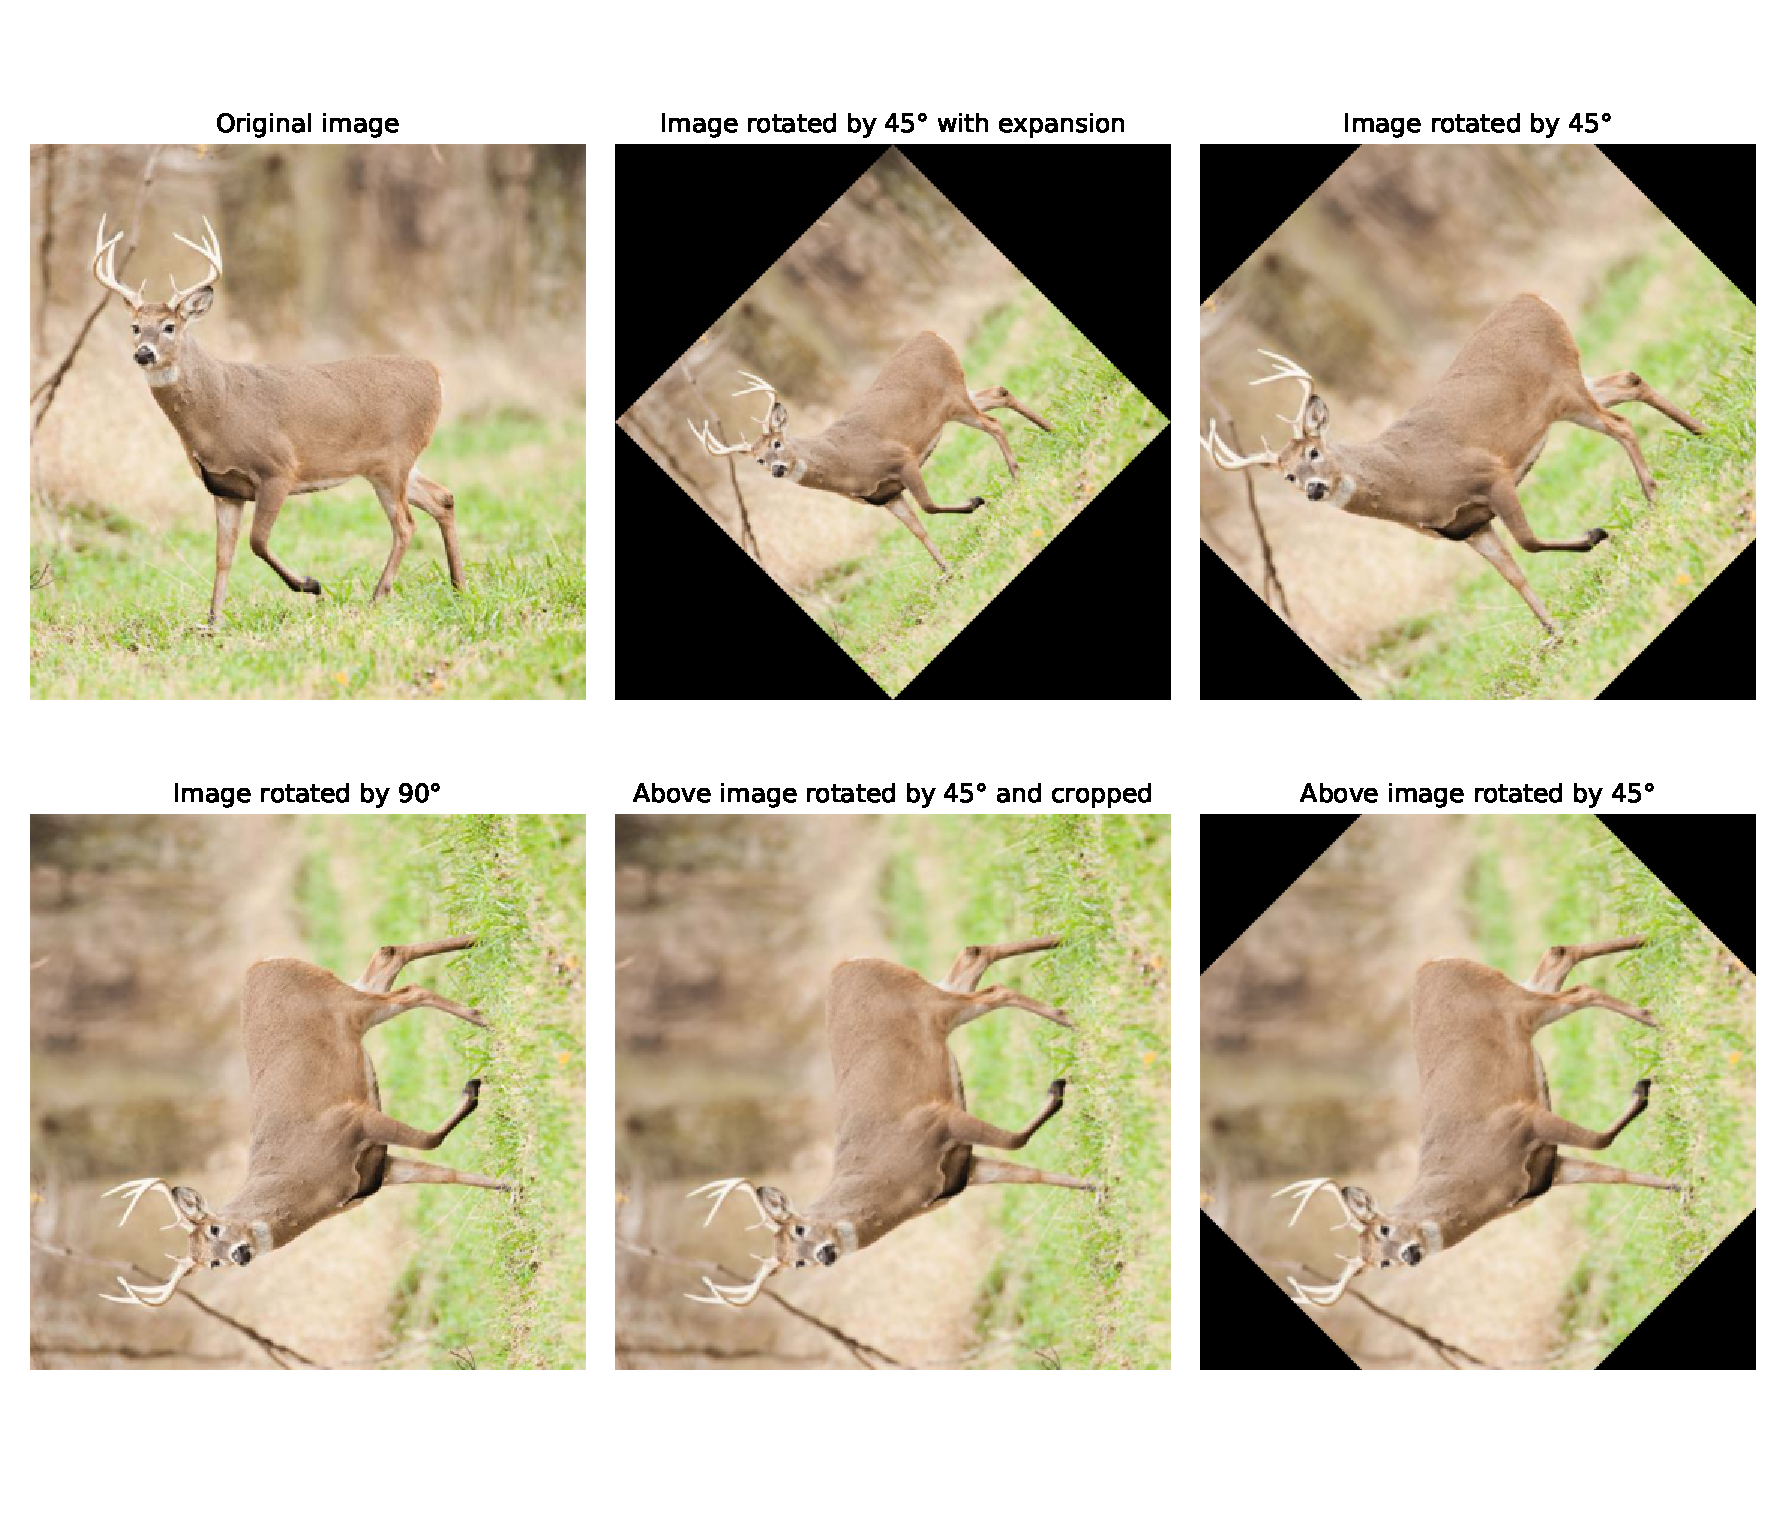
\includegraphics[width=\textwidth]{rotations}
            \label{fig:rotation_pics}
            \caption{Difference between rotation with and without border
                expansion. Left column shows the original image and it's
                rotation by 90\degree. In middle column image is first rotated
                by 45\degree with expansion, then rotated again and cropped to
                original size. In the right column picture is simply rotated
                twice by 45\degree.}
        \end{figure}
        While filters present in GCNNs are higher dimensional than in regular
        CNNs, spatial interpretation of the last two dimensions remains
        unchanged. Therefore it makes sense to generalize $\mathcal{R}$ to
        transform N-dimensional tensor by separetely rotating last two
        dimensions of every subtensor and stacking them in original shape.
        The same goes for scaling and shear transformations described next.

    \subsubsection{Scaling}
        Scaling is a zoom-in or zoom-out transformation in reference to the
        center of the image. Scaling of cooridnates can be written as
        \begin{equation}
            \mathcal{S}_k = \begin{bmatrix}
                k & 0 \\
                0 & k
            \end{bmatrix}
        \end{equation}
        Just like in rotation, after rescaling of coordinates, image needs to be
        resampled.
        Figure \ref{fig:scalings} shows varying degree of scaling.
        Note that by default scaling-up causes loss of
        information, so we might want to use image expansion as well.
        However while using finite expansion (increasting image size by at most
        $\sqrt{2}$) we can make rotations into a group action,
        it's not the case for scaling. In order to preserve all information
        during scaling by factor of $k>1$, we would have to increase image
        size by the same factor. For this reason scaling is often modeled not as
        a group, but rather as a semi-group or monoid. However it's not really any
        obstacle -- what matters is that locally it still has structure of a Lie
        group.


        \newcommand{\scalepic}[2]{
            \begin{subfigure}{#2\textwidth}
                \includegraphics[width=\linewidth]{{scalings/#1}.jpg}
            \end{subfigure}}
        \newcommand{\scalepiccaption}[3]{
            \begin{subfigure}{#2\textwidth}
                \includegraphics[width=\linewidth]{{scalings/#1}.jpg}
                \caption*{$k=#3$}
            \end{subfigure}}

        \begin{figure}[h]
            \centering
            \foreach \n in {0.5,0.75,1,1.5,2}
                {\scalepic{0temp\n}{0.18}} \\
            \foreach \n in {0.5,0.75,1,1.5,2}
                {\scalepic{121temp\n}{0.18}} \\
            \foreach \n in {0.5,0.75,1,1.5,2}
                {\scalepiccaption{105temp\n}{0.18}{\n}}

            \caption{Images from STL10 dataset with scaled by a factor of $k$.}
            \label{fig:scalings}
        \end{figure}

    \subsubsection{Shear}
        Shear operator `tilts' the coordinates. If we use the standard coordinate
        system centered  in the middle of the image,
        the first vector $e_1$ remains unchanged while $e_2$ is mapped
        to $\lambda e_1 + e_2$:
        \begin{equation}
        \mathcal{SH}_\lambda = \begin{bmatrix}
                1 & \lambda \\
                0 & 1
            \end{bmatrix}
        \end{equation}
        where $\lambda \in \mathbb{R}$. Parameter $\lambda$ is theoretically
        unbounded so the remarks from scaling section apply here as well. In
        practice however $\lambda = \pm -1$ causes tilt of $45 \degree$ which is
        already very significant so we only consider $\lambda \in [-1;1]$.
        Exemplary effect of transformation is shown in figure \ref{fig:shears}.

        \newcommand{\shearpic}[2]{
            \begin{subfigure}{#2\textwidth}
                \includegraphics[width=\linewidth]{{shears/#1}.jpg}
            \end{subfigure}}
        \newcommand{\shearpiccaption}[3]{
            \begin{subfigure}{#2\textwidth}
                \includegraphics[width=\linewidth]{{shears/#1}.jpg}
                \caption*{$\lambda=#3$}
            \end{subfigure}}

        \begin{figure}[h]
            \centering
            \foreach \n in {-1,-0.5,0,0.5,1}
                {\shearpic{0temp\n}{0.18}} \\
            \foreach \n in {-1,-0.5,0,0.5,1}
                {\shearpic{121temp\n}{0.18}} \\
            \foreach \n in {-1,-0.5,0,0.5,1}
                {\shearpiccaption{105temp\n}{0.18}{\n}}

                \caption{Images from STL10 dataset transformed by
                $\mathcal{SH}_\lambda$ for varying $\lambda$.}
            \label{fig:shears}
        \end{figure}

